\section{Methodology and Implementation}
The implementation consists of continuous regression modeling with spatial and temporal validation, recursive daily future forecasting, unmonitored location spatial estimation, and multi-class AQI classification. Fig. \ref{fig:workflow_diagram} illustrates our end-to-end processing pipeline.

\begin{figure}[htbp]
\centering
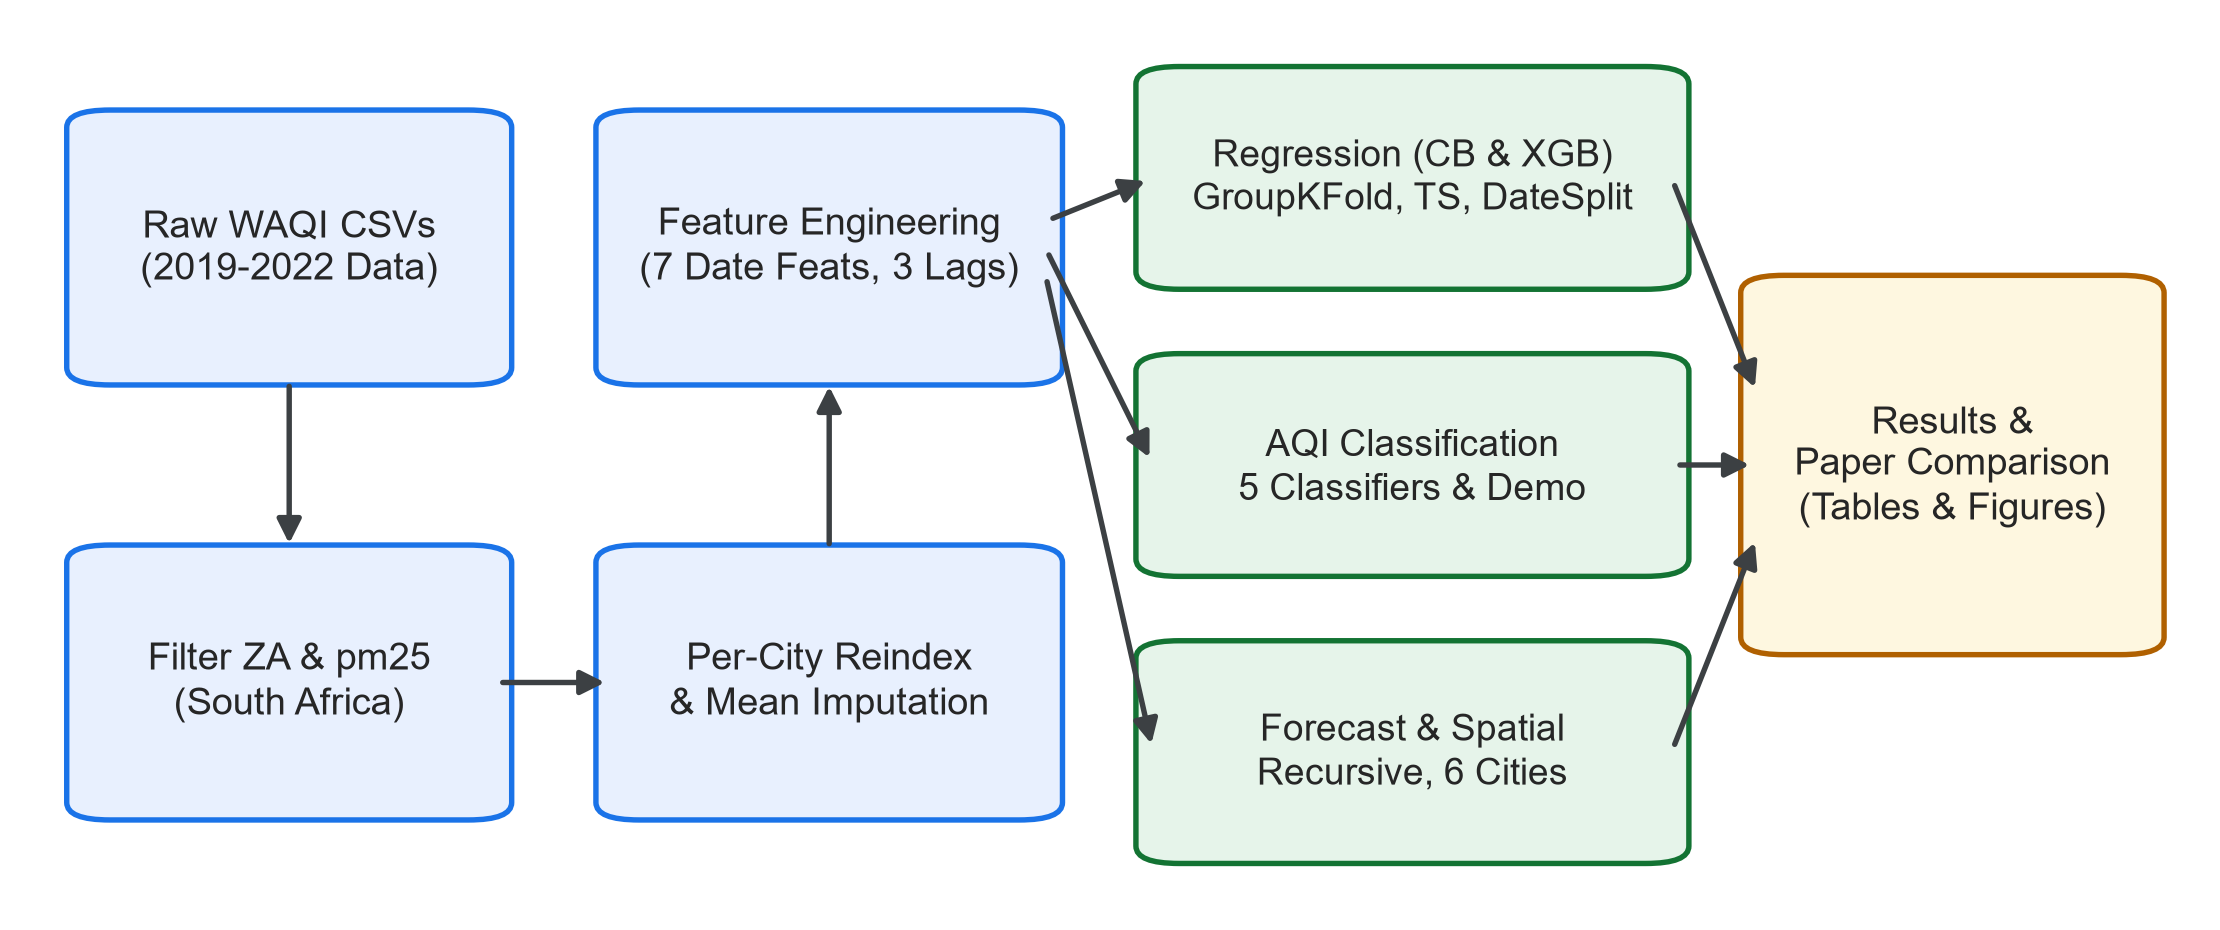
\includegraphics[width=0.92\linewidth]{figures/figure1_workflow.png}
\caption{End-to-End System Workflow Architecture for the South Africa PM2.5 Prediction Pipeline.}
\label{fig:workflow_diagram}
\end{figure}

\subsection{Gradient Boosting Regression Models}
We implemented two gradient boosted regression algorithms: \textbf{CatBoost Regressor} \cite{prokhorenkova2018catboost}, configured with 1,000 iterations, RMSE loss function, early stopping patience of 100 iterations, and random seed 42; and \textbf{XGBoost Regressor} \cite{chen2016xgboost}, initialized with a base score of 0.5, booster \texttt{gbtree}, squared error objective, learning rate of 0.01, maximum tree depth of 3, 1,000 estimators, and early stopping patience of 50 rounds. In each cross-validation fold, the held-out validation set was passed to monitor loss. Because the held-out fold was also used as the validation set for early stopping, the reported cross-validation RMSE can be slightly optimistic.

\subsection{Cross-Validation Protocols}
We evaluated two cross-validation schemes:
\begin{itemize}
    \item \textbf{Primary Spatial Cross-Validation}: The base paper evaluated five steps with training city counts of 9, 9, 10, 10, and 10. Our spatial cross-validation with \texttt{GroupKFold(n\_splits=5)} yielded training city counts of 10, 10, 9, 9, and 10 per fold; these counts match the paper's set of split sizes, but they occur in a different fold order because scikit-learn assigns whole groups to folds by group size, and we do not claim the same fold order. Because entire cities are placed in the test split, the model predicts for locations withheld from training. However, because each city's records retain their own historical \texttt{lag1}, \texttt{lag2}, and \texttt{lag3} values, the model still receives location-specific past sensor signals. Therefore, this protocol does not represent pure spatial generalization to locations without any prior sensor history.
    \item \textbf{Secondary Temporal Cross-Validation}: We applied \texttt{TimeSeriesSplit} (5 splits, 150-day test window, 24-day gap) independently to each city's time series to measure chronological forecasting performance within established stations.
\end{itemize}

\subsection{Multi-Step Recursive Forecasting and Spatial Interpolation}
For future forecasting, we trained models on records up to November 25, 2022, and generated daily predictions through December 31, 2023 (401 days). We implemented a recursive simulation: on each day, model predictions were dynamically inserted into the history to supply subsequent lag values (\texttt{lag1}, \texttt{lag2}, \texttt{lag3}). To sanity-check the forecast, we evaluated predictions against actual sensor readings from November 26, 2022 to December 31, 2022 where ground data was available.

For the six unmonitored municipalities, we trained on all twelve monitored stations using latitude, longitude, and calendar features, and predicted daily 2022 values. We assessed spatial coordinate interpolation using Leave-One-City-Out (LOCO) cross-validation across the twelve monitored stations.

\subsection{Air Quality Index Classifiers}
We implemented the five supervised classifiers evaluated in the base paper: Random Forest, Logistic Regression, Support Vector Machine (SVC with RBF kernel), K-Nearest Neighbors ($k = 5$), and Decision Tree. Following the paper's design, each model received only a single input feature, \texttt{Median\_PM25}, and predicted one of the six discrete US EPA AQI classes: Good ($0$), Moderate ($1$), Unhealthy for Sensitive Groups ($2$), Unhealthy ($3$), Very Unhealthy ($4$), and Hazardous ($5$).
